% This is the aspauthor.tex LaTeX file
% Copyright 2010, Astronomical Society of the Pacific Conference Series

\documentclass[11pt,twoside]{article}
\usepackage{graphicx}
\usepackage{asp2010}
\resetcounters
\bibliographystyle{asp2010}

\markboth{A. Schaaff, T. Boch, P. Fernique, R. Houpin, V. Kaestl\'e, M. Royer, J. Scheffmann, A. Weiler}{A. Schaaff, T. Boch, P. Fernique, R. Houpin, V. Kaestl\'e, M. Royer, J. Scheffmann, A. Weiler}

\begin{document}

\title{Feedback about astronomical application developements for mobile devices}
\author{A. Schaaff$^1$, T. Boch$^2$, P. Fernique$^2$, R. Houpin$^4$, V. Kaestl\'e$^3$, M. Royer$^4$, J. Scheffmann$^4$, A. Weiler$^4$
\affil{$^1$CDS, CNRS, Observatoire astronomique, 11 rue de l'Universit\'e 67000 Strasbourg}
\affil{$^2$CDS, UDS,  Observatoire astronomique, 11 rue de l'Universit\'e 67000 Strasbourg}
\affil{$^3$Universit\'e de Strasbourg,  67000 Strasbourg}
\affil{$^4$Universit\'e de Lorraine, 54000 Nancy}}

\begin{abstract}
Within a few years, Smartphones have become the standard for mobile telephony, and we are now witnessing a rapid development of Internet tablets. These mobile devices have enough powerful hardware features to run more and more complex applications. In the field of astronomy it is possible to use these tools to access data via a simple browser, but also to develop native applications reusing libraries (Java for android, Objective-C for iOS) developed for desktops. We are working since two years on mobile application development and we have now skills in native iOS and Android developments, Web development (especially HTML5, JavaScript, CSS3) and conversion tools (PhoneGap) from Web development to native applications. The biggest change comes from human/computer interaction that is radically changed by the use of multitouch. This interaction requires a redesign of interfaces to take advantage of new features (simultaneous selections in different parts of the screen, etc.). In the case of native applications, the distribution is usually done through online stores (App Store, Google Play, etc..) which gives a visibility to a wider audience. Our approach is to perform testing of materials, development of prototypes but also operational applications. The native application development is costly in development time, but the possibilities are broader because it is possible to use for example the gyroscope and the accelerometer, to point an object in the sky. Developments depend on the Web browser and the rendering and performance are often very different. It is also possible to convert Web developments to native applications, but currently it is better to restrict this possibility to light applications in terms of functionality. Developments in HTML5 are promising but are far behind those available on desktops. HTML5 has the advantage of allowing developements independent from the evolution of the mobile platforms ("write once, run everywhere"). The upcoming of Windows 8 supported on desktops, Internet tablets as well as a mobile version for smartphones will further expand the native systems family. This will enhance the interest of Web development.
\end{abstract}

\section{Introduction}
In 2010, we started to develop for Android with a prototype based on VizieR Mine. In 2011 we developed SkySurveys, which reuses HEALPix Java libraries from Aladin. It lets you navigate through surveys. It also uses the OpenGL library. In 2012 we developed SkyObjects natively for iOS and Android. This application provides information about astronomical objects, stores them locally with the user own information and points the objects in the sky, etc. We also tested the same type of application with HTML5 and we are working to improve its display performance. SkyObjects is in the deposit process on Google Play and on the App Store. SkySurveys is available directly from the CDS Web pages. We will present these developments with a critical eye.

\section{Differents ways of developments}

We have explored three ways to build applications for mobile devices.
It is possible to develop Web application in HTML4/5 like for desktops but with dedicated Javascript libraries like Mobile jQuery which are optimized for mobile devices.
A second solution is to develop a native application in Java for Android, Objective C for iOS, etc. 
A third solution is to develop Web applications in HTML and javascript and to convert these applications in pseudo native applications through converters like PhoneGap.
We have not tried an another way which consist in the developement in one language (for example Java) and the conversion to an another like Objective-C. It is possible to find a few frameworks to do it like J2ObjC which converts just the Java code (data access, etc.) excepted the GUI side.

\subsection{Web developements}
Web develpoment is the fastes way to develop an application on mobile devices. A several number of frameworks and javascript librariries are now available and it is possible to create a very nice application in a few hours or at least in a few days for a well designed application.
A mobile version of the CDS Portal has been developed through this way (see Fig.~\ref{O28:1}).

\begin{figure}[h] \center
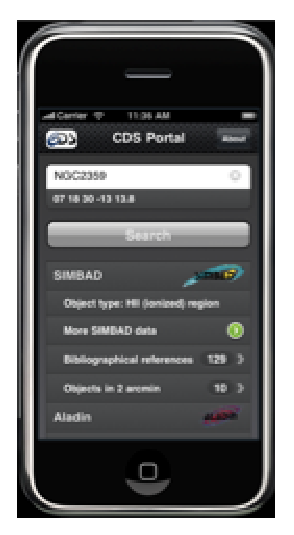
\includegraphics[scale=0.7]{O28_f4.eps}
\caption{CDS mobile portal} 
\label{O28:1}
\end{figure}

\subsection{Native developements}
The number of HEALpix (\citep{gorski_2005}) available surveys is growing and a few HEALPix visualizer are available like Aladin through the Allsky mode (\citep{fernique_2010}). This mode runs well on a desktop or a laptop with good performances and it was a real challenge to develop a visualizer for smartphones and Internet tablets. We decided to develop it on android because it was possible to reuse a part of the Aladin sources written in Java. The first tests were not really good due to the basic hardware capabilities compared to a desktop. Aladin does not use OpenGL but this graphical library is available on almost all the mobile devices. The new prototype implementing this library was between thirty and fourty times faster and the FPS (frames per second) were suffisant to provide a fluid display.
All the surveys available and added in the future in Aladin will also be available in the application called SkySurveys (see Fig.~\ref{O28:2}). It is possible to try it by downloding on the CDS developer's corner. 
We consider this application as an advanced prototype for android devices and we will probably not develop the same on iOS devices.

\begin{figure}[h] \center
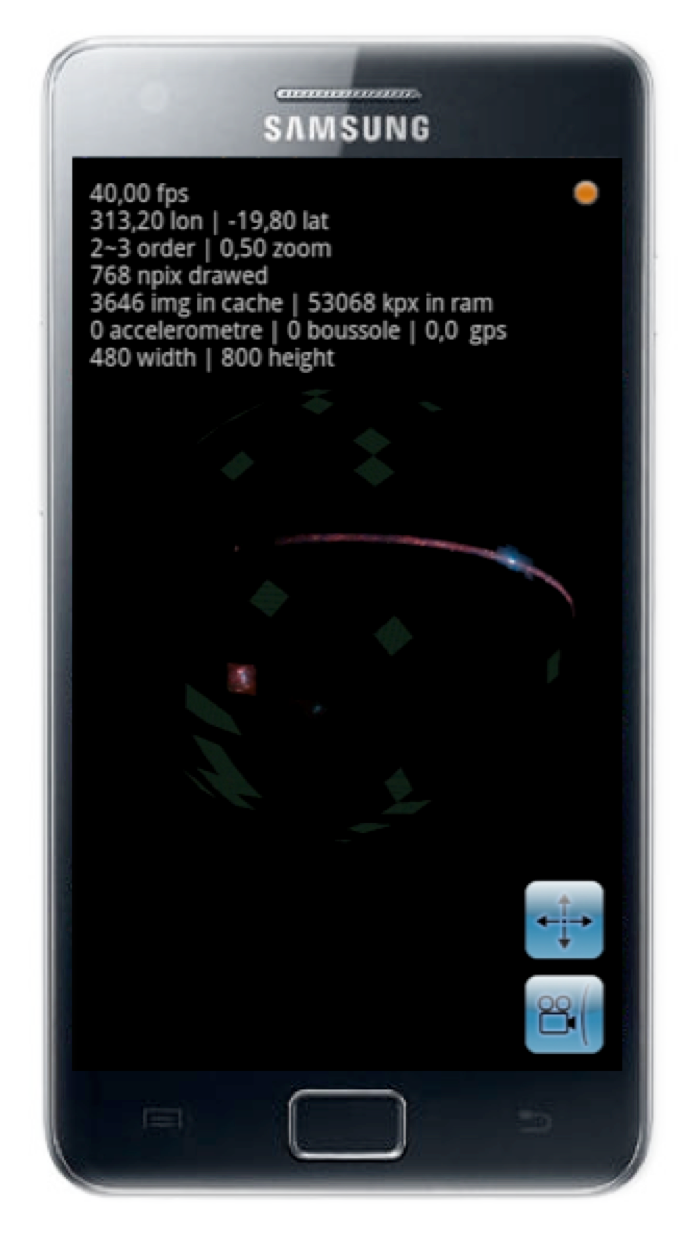
\includegraphics[scale=0.28]{O28_f1.eps}
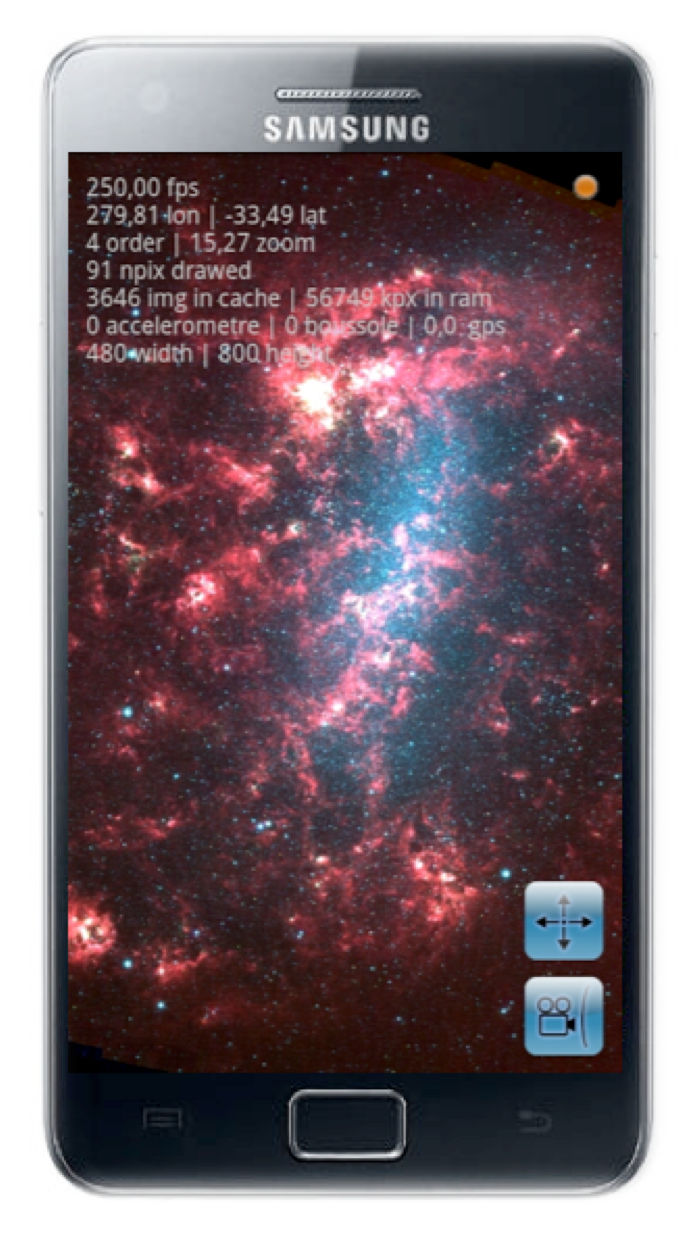
\includegraphics[scale=0.28]{O28_f2.eps}
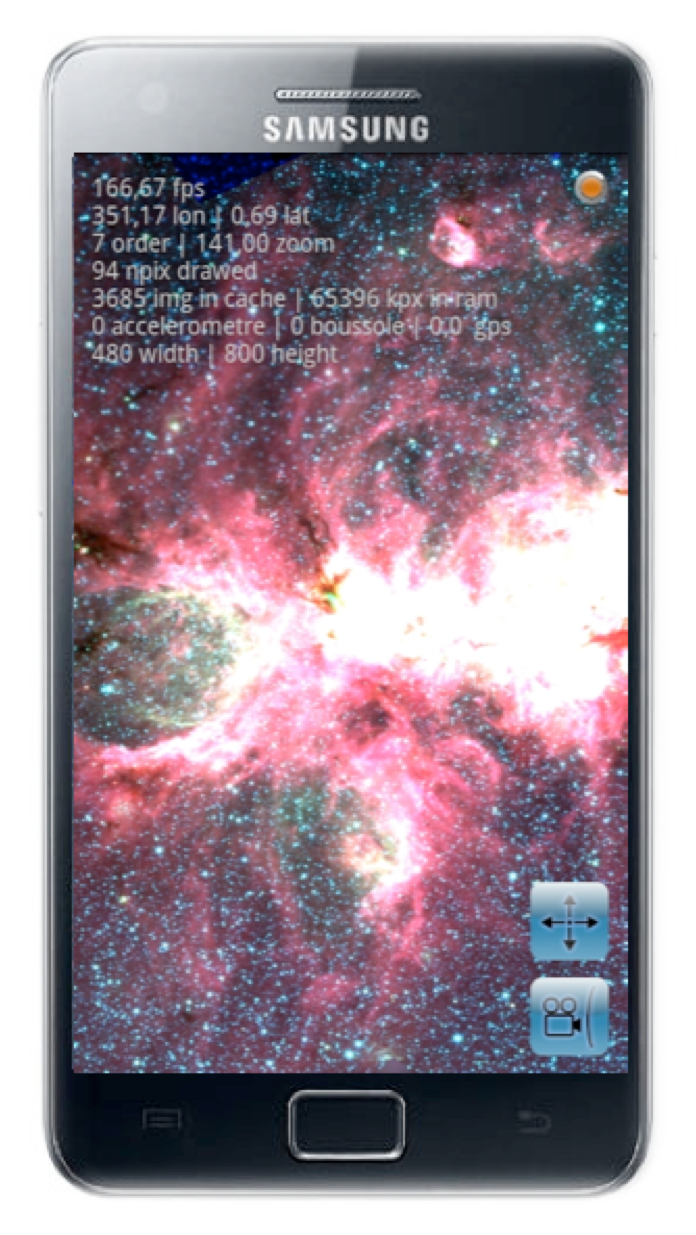
\includegraphics[scale=0.28]{O28_f3.eps}
\caption{Spitzer survey (credits JPL/NASA)} 
\label{O28:2}
\end{figure}

\subsection{Converters}
We have developped the main features of SkyObjects in HTML5 and we have convert it using PhoneGap to iOS and android applications. But we had at least a big "gap" between the final application and what we had developed directly in Java or Objective-C : the generated application is not a real native application, it is just an android or iOS application implementing an HTML5 emulator with the HTML5 Web application code. So it is not a real conversion to a native langage... 
It means also that it is not possible to convert in a native langage and to modify this code.
An another difficulty was also the lack of some functionalities od the mobile devices like the gyroscope  (see Fig.~\ref{O28:3}).

\begin{figure}[h] \center
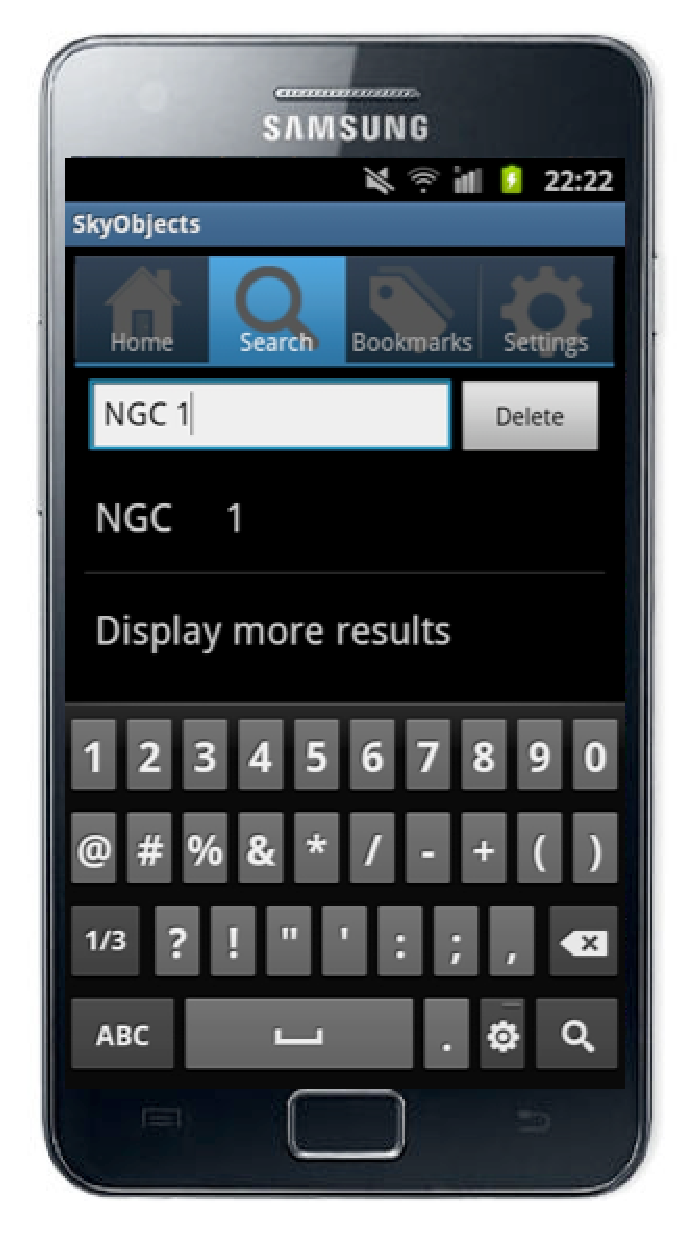
\includegraphics[scale=0.28]{O28_f5.eps}
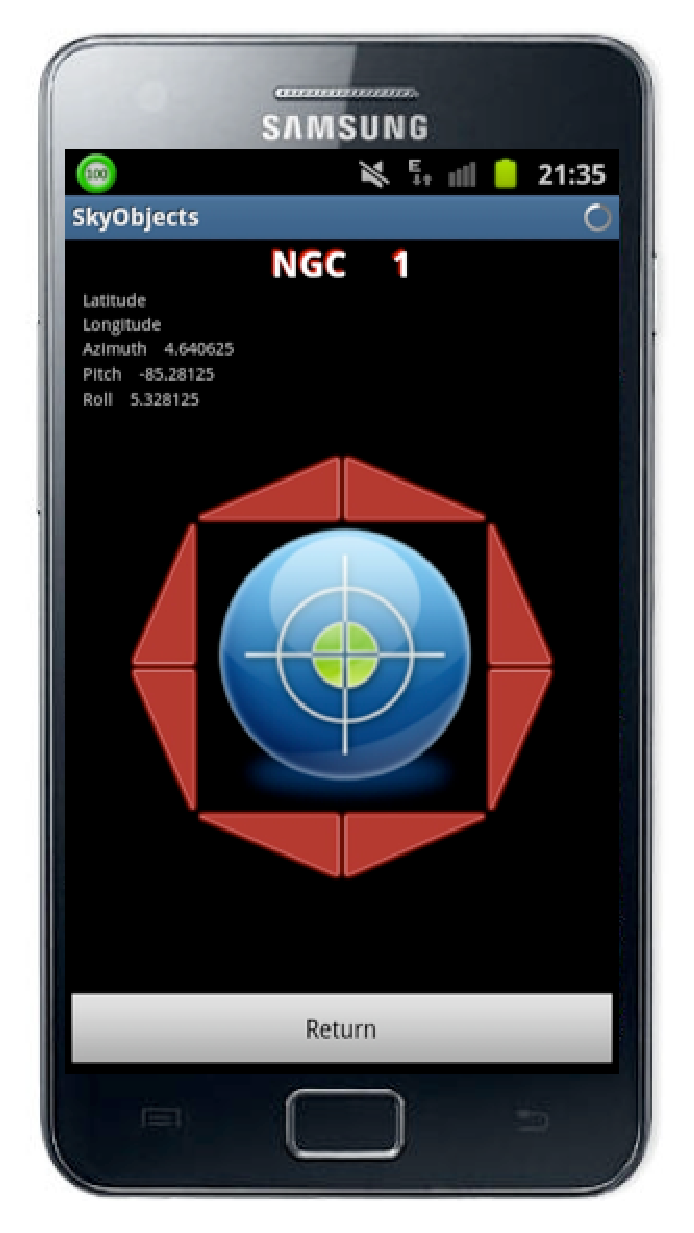
\includegraphics[scale=0.28]{O28_f6.eps}
\caption{SkeySurveys with pointing functionality using gyroscope, ...} 
\label{O28:3}
\end{figure}

\section{Perspectives}
We are now focusing the new developments on Web apps based on HTML5 (\url{http://www.w3.org/TR/html5/}), which can provide rich content and which should become a standard probably in around one year. As it is not easy to have both Java and Objective-C skills in a team and to have enough time for native developements, it has the advantage of allowing developments independent of the mobile platform and to avoid the deep tests which are needed for example on android devices. 
But frameworks should also evolved and it should be easier in the future to develop applications for the main mobile operating systems without doing the work two or three times.
All the experiments are detailed at \url{http://http://cds.u-strasbg.fr/resources/doku.php?id=mobiledev}.

\section{Conclusion}
This first prototypes were important to evaluate the time necessary to develop tools for mobile devices and to have a reflexion about which service or application would be useful on this kind of devices. The developement of native applications for mobile devices has a high cost less in term of man power and time. It is easy to use for example existing Java source code with a quick development of an Android user interface but development from scratch needs a time silimar to a development for desktops or laptops. We think that the development of an native "app" for Android or iOS are justified if it is not possible to provide or adapt a simple Web application (HTML and Javascript)  independant from the device.

\bibliography{O28}

\end{document}
